\documentclass[UTF-8,twoside,c5size]{ctexart}
\usepackage[dvipsnames]{xcolor}
\usepackage{amsmath}
\usepackage{amssymb}
\usepackage{geometry}
\usepackage{listings}
\usepackage{setspace}
\usepackage{xeCJK}
\usepackage{ulem}
\usepackage{pstricks}
\usepackage{pstricks-add}
\usepackage{bm}
\usepackage{mathtools}
\usepackage{breqn}
\usepackage{mathrsfs}
\usepackage{esint}
\usepackage{textcomp}
\usepackage{upgreek}
\usepackage{pifont}
\usepackage{tikz}
\usepackage{circuitikz}
\usepackage{caption}
\usepackage{tabularx}
\usepackage{array}
\usepackage{pgfplots}
\usepackage{multirow}
\usepackage{pgfplotstable}
\usepackage{mhchem}
\usepackage{graphicx}

\newcolumntype{Y}{>{\centering\arraybackslash}X}
\geometry{a4paper,centering,top=1.27cm,bottom=2.54cm,left=2cm,right=2cm}
\graphicspath{{figures/}}
\pagestyle{plain}
\captionsetup{font=small}

%\CTEXsetup[name={,.}]{section}
\CTEXsetup[format={\raggedright\heiti\noindent\zihao{-3}},numberformat={\bfseries}]{section}
\CTEXsetup[format={\raggedright\heiti\zihao{4}},numberformat={\bfseries}]{subsection}
\CTEXsetup[format={\raggedright\heiti\quad\zihao{-4}},numberformat={\bfseries}]{subsubsection}
\CTEXsetup[format={\raggedright\heiti\qquad},numberformat={\bfseries}]{paragraph}
\CTEXsetup[beforeskip=1.0ex plus 0.2ex minus .2ex, afterskip=1.0ex plus 0.2ex minus .2ex]{paragraph}
\renewcommand\thefootnote{\ding{\numexpr171+\value{footnote}}}

\setstretch{1.5}

\setCJKfamilyfont{boldsong}[AutoFakeBold = {2.17}]{SimSun}
\newcommand*{\boldsong}{\CJKfamily{boldsong}}
%\DeclareMathOperator\dif{d\!}
\newcommand*{\me}{\mathop{}\!\mathrm{e}}
\newcommand*{\mpar}{\mathop{}\!\partial}
\newcommand*{\dif}{\mathop{}\!\mathrm{d}}
\newcommand*{\tab}{\indent}
\newcommand*{\mcelsius}{\mathop{}\!{^\circ}\mathrm{C}}
\renewcommand*{\Im}{\mathrm{Im}\,}

\setcounter{secnumdepth}{4}

\renewcommand\arraystretch{1.5}

\lstset{
	backgroundcolor=\color[RGB]{245,245,245},
	keywordstyle=\color{blue}\bfseries,
	basicstyle=\small\ttfamily,
	commentstyle=\itshape\color{olive},
	numberstyle=\ttfamily,
	tabsize=4,
	breaklines=true
}

\begin{document}
	\begin{center}
		\heiti\zihao{-2}
		实验\textbf{6}报告
	\end{center}

	\begin{table*}[!h]
		\raggedleft
		\zihao{-4}
		\begin{tabular}{ccc}
			{\heiti 学号} & {2019K8009929019} & {2019K8009929026} \\
			{\heiti 姓名} & 桂庭辉 & 高梓源 \\
			{\heiti 箱子号} & \multicolumn{2}{c}{44}
		\end{tabular}
	\end{table*}
	
	\section{实验任务}
	
	本次实验在流水线中添加部分普通用户态指令,主要包括9条算术逻辑运算类指令和7条乘除运算类指令。由于实现的指令主要针对运算,故而主要的实现基于已有的流水线框架与已实现指令的数据通路即可,较为复杂的处理在乘除法指令上。
	
	\section{实验设计}	
	
	\subsection{总体设计思路}
	
	9条算术逻辑运算类指令的实现主要复用此前流水线中已实现的部分指令功能。\texttt{slti, sltui, andi, ori, xori}指令分别复用\texttt{slt, sltu, and, or, xor}指令数据通路,处理立即数内容与相关控制信号即可。\texttt{sll, srl, sra}指令分别复用\texttt{slli, srli, srai}指令数据通路,调整操作数来源与相关控制信号即可。\texttt{pcaddu12i}指令主要通路复用\texttt{add}指令,操作数处理上来自PC寄存器与\texttt{lu12i}指令结果。由于此部分几乎全部为对已有数据通路的复用,仅添加了部分控制信号,故而本篇报告中不再详述该部分的实现细节。
	
	7条乘除法运算类指令中,乘法的处理我们使用自己编写的流水化乘法器,在两拍内计算出乘法结果;除法与取模的处理我们选择调用Xilinx IP定制除法器运算部件进行实现。具体运算的进行在ALU部件中完成,由于引入了新的运算与相关控制信号,需要维护流水级间的寄存器宽度、\texttt{alu\_op}宽度以及流水线控制的部分信号。
	
	\subsection{重要模块设计:mul\_top与流水化后乘法实现}
	本小节所有模块设计均在tools.v文件中。
	\subsubsection{功能描述}
	
	乘法器顶层模块,例化17个数相加华莱士树模块\texttt{wallace}与33位Booth两位乘部分积生成器\texttt{boothgen}完成乘法器整体搭建与流水化。
	
	\subsubsection{工作原理}
	
	考虑硬件资源的节省,本次设计一个乘法器以完成有符号与无符号32位补码乘法。实现上如实验讲义所说将输入扩展成33位,通过33位补码乘法器实现对有无符号运算的同时支持。整体结构同样来自实验讲义。
	
	Booth两位乘部分积生成器的设计来自理论课教材,17个数相加的华莱士树设计来自实验课讲义。此处均不再赘述。在流水级划分上,考虑Booth部分积生成逻辑与华莱士树中6层1位全加器的总延迟约为20余级门(具体延迟大小取决于Vivado对1位加法器的实现),最终合并华莱士树结果的66位加法器将产生相当级别的延迟,故而选择将流水级切分在66位加法器入口处实现。采用一个133位寄存器将加法器的两个66位输入与1位进位输入锁一拍以实现流水化,在两拍内计算得到乘法结果。
	
	流水化的主要实现如下:
	\begin{lstlisting}[language=verilog]
	reg [132:0] bus;
	
	always @ (posedge clk) begin
		if (rst) begin
			bus <= 133'b0;
		end else begin
			bus <= {add_src1, add_src2, c[15]};
		end
	end
	
	assign res = bus[132:67] + bus[66:1] + {65'b0, bus[0]};\end{lstlisting}
	
	\subsubsection{接口定义}
	
	接口定义见下页。
	
	\begin{table}[!h]
		\centering
		\caption{乘法器顶层模块接口}
		\begin{tabularx}{\textwidth}{|c|c|c|Y|}
			\hline
			\textbf{名称} & \textbf{方向} & \textbf{位宽} & \textbf{描述} \\
			\hline
			\texttt{clk} & \textsc{In} & 1 & 时钟信号 \\
			\hline
			\texttt{rst} & \textsc{In} & 1 & 复位信号,高电平有效 \\
			\hline
			\texttt{mul\_signed} & \textsc{In} & 1 & 是否做有符号乘法 \\
			\hline
			\texttt{src1} & \textsc{In} & 32 & 源操作数1 \\
			\hline
			\texttt{src2} & \textsc{In} & 32 & 源操作数2 \\
			\hline
			\texttt{res} & \textsc{Out} & 64 & 乘法运算结果 \\
			\hline
		\end{tabularx}
	
		\caption{华莱士树模块接口}
		\begin{tabularx}{\textwidth}{|c|c|c|Y|}
			\hline
			\textbf{名称} & \textbf{方向} & \textbf{位宽} & \textbf{描述} \\
			\hline
			\texttt{in} & \textsc{In} & 17 & 待相加的17个1位数 \\
			\hline
			\texttt{cin} & \texttt{In} & 14 & 来自先前华莱士树或转置部件的进位输入 \\
			\hline
			\texttt{cout} & \textsc{Out} & 14 & 传递给后续华莱士树的进位输入 \\
			\hline
			\texttt{carry} & \textsc{Out} & 1 & 压缩结果:进位输出 \\
			\hline
			\texttt{sum} & \textsc{Out} & 1 & 压缩结果:和 \\
			\hline
		\end{tabularx}
	
		\caption{部分积生成模块接口}
		\begin{tabularx}{\textwidth}{|c|c|c|Y|}
			\hline
			\textbf{名称} & \textbf{方向} & \textbf{位宽} & \textbf{描述} \\
			\hline
			\texttt{y} & \textsc{In} & 3 & 来自乘数的部分积生成标志信号 \\
			\hline
			\texttt{x} & \textsc{In} & 66 & 移位处理后的被乘数 \\
			\hline
			\texttt{c} & \textsc{Out} & 1 & 部分积的末位进位输入(取反“加一”) \\
			\hline
			\texttt{p} & \textsc{Out} & 66 & 部分积 \\
			\hline
		\end{tabularx}
	\end{table}

	\subsubsection{乘法实现的其他逻辑}
	
	由于乘法器与其他运算逻辑一样集成到ALU部件中,而流水化后的乘法指令为了避免影响流水线性能,应如访存指令一样在指令进入流水级时取得乘法结果,为了实现该功能,需要将乘法运算结果导出至执行级外传递给访存级。乘法实现里引入的时序逻辑除此前介绍的乘法计算中的流水级切分外,乘法所需结果是高32位还是低32位所需的控制信号也需要时序逻辑保存到下一拍,即乘法指令位于访存级时。该信号的传递可以通过执行级与访存级间的流水槽实现,也可以单独缓存该信号利用传递乘法结果的通路进入访存级参与结果选择。
	
	此外,由于乘法指令与访存指令一样,在访存级才能得到写回结果,故而如访存指令一样,也需在前递机制中引入乘法指令于执行级与译码级指令冲突时的阻塞信号。
	
	\subsection{除法器IP调用与时序处理}
	
	笔者将乘除法所有实现放在alu.v中,这就意味着alu\_op需要拓宽至19位,囊括所有乘除法指令信息,对于除法需要有无符号的信息、取商或余数的信息,并且这些信息彼此互斥,很难提取共同特征而缩减,因此可直接对乘除法每类指令设置一位alu\_op,求得的结果也可以根据alu\_op直接选取。
	
	\subsubsection{接口定义}
	
	根据讲义描述,调用并设置好Vivado提供的有无符号除法IP核,注意IP核暴露的所有接口都有作用,需要全部连接,接口如下页。
	
	\begin{table}[!h]
	\begin{center}
		\caption{除法器IP核接口定义}
		\begin{tabularx}{\textwidth}{|c|c|c|Y|}
			\hline
			\textbf{接口} & \textbf{I/O} & \textbf{位宽} & \textbf{说明} \\
			\hline
			\texttt{aclk} & \textsc{In} & 1 & 时钟驱动,迭代除法 \\
			\hline
			\texttt{s\_axis\_divisor\_tdata} & \textsc{In} & 32 & 除数输入 \\
			\hline
			\texttt{s\_axis\_dividend\_tdata} & \textsc{In} & 32 & 被除数输入 \\
			\hline
			\texttt{s\_axis\_divisor\_tready} & \textsc{Out} & 1 & 是否准备好读取除数 \\
			\hline
			\texttt{s\_axis\_dividend\_tready} & \textsc{Out} & 1 & 是否准备好读取被除数 \\
			\hline
			\texttt{s\_axis\_divisor\_tvalid} & \textsc{In} & 1 & 除数输入是否有效,开始运算 \\
			\hline
			\texttt{s\_axis\_dividend\_tvalid} & \textsc{In} & 1 & 被除数输入是否有效,开始运算 \\
			\hline
			\texttt{m\_axis\_dout\_tdata} & \textsc{Out} & 64 & 商和余数结果输出 \\
			\hline
			\texttt{m\_axis\_dout\_tvalid} & \textsc{Out} & 1 & 输出是否有效,当前除法是否算完 \\
			\hline
		\end{tabularx}
	\end{center}
	\end{table}

	\subsubsection{使用说明}
	\label{Valid_input}

	正如讲义强调的,除法IP核采用AXI总线接口,Ready和Valid信号同时有效时开始输入,经过观察,我们设置的clocks per Division选项是Ready信号每次拉高间隔的时钟周期数,我们需要保证Valid信号第一次和Ready信号同时拉高后必须在该除法计算整个完成后(m\_axis\_dout\_tvalid信号拉高)之后才能有条件再度拉高,进行下一次计算,在此过程中流水级也需要进行阻塞。
	
	笔者在实验中使用了另一个信号div\_valid,它为高电平当且仅当整个除法运算开始且未结束,于是一旦它为高电平,除法器输入的两个Valid信号就不能拉高。因为除数被除数的Ready和Vallid信号需要同时拉高,用同一个div\_data\_valid信号进行控制即可,于是下面是控制信号的时序赋值过程:
	
	\begin{lstlisting}[language=verilog]
	always @(posedge clk) begin
		if (div_valid) begin
			div_data_valid <= 1'b0;
		end else if (es_valid & use_div & (~divisor_data_ready | ~dividend_data_ready)) begin
			div_data_valid <= 1'b1;
		end else begin
			div_data_valid <= 1'b0;
		end
		
		if (div_valid) begin
			divu_data_valid <= 1'b0;
		end else if (es_valid & use_divu & (~u_divisor_data_ready | ~u_dividend_data_ready)) begin
			divu_data_valid <= 1'b1;
		end else begin
			divu_data_valid <= 1'b0;
		end
		
		if (rst) begin
			div_valid <= 1'b0;
		end else if (div_res_valid | divu_res_valid) begin
			div_valid <= 1'b0;
		end else if ((div_data_valid & divisor_data_ready) | (divu_data_valid & u_divisor_data_ready)) begin
			div_valid <= 1'b1;
		end
	end
	\end{lstlisting}

	除法器实例化连接后,对于结果直接取$[63:32]$位作为商,$[31:0]$作为余数。
	
	\section{实验过程}
	
	\subsection{实验流水账}
	
	2021.09.30 08:00 $\sim$ 2021.09.30 09:00 :完成第一部分,对9条算术逻辑类指令的实现
	
	2021.10.01 14:00 $\sim$ 2021.10.01 16:00 :利用Xilinx IP完成乘除法指令实现
	
	2021.10.02 15:00 $\sim$ 2021.10.02 16:45 :完成流水化乘法器支持乘法指令
	
	2021.10.02 18:00 $\sim$ 2021.10.03 00:00 :撰写实验报告
	
	\subsection{错误记录}	
	\subsubsection{错误\textbf{1:}流水化后乘法结果获取出错}
	\paragraph{错误现象}\hfill
	
	%	四级节标题后面的\hfill与空行不可省略,不然节内容会跟着标题,目前我也只会这方法处理
	
	对于乘法指令,在访存级获取到的计算结果为0。
	
	\paragraph{分析定位过程}\hfill
	
	无论是访存级还是执行级,其中获取到的乘法结果均为0,但乘法器结果正确,说明问题来自ALU中对乘法结果的处理。
	
	\paragraph{错误原因}\hfill
	
	在最初的设计中,我们在ALU中根据\texttt{alu\_op}译码结果对乘法结果的高低位进行选择,然后传递32位数据给访存级,这一过程的“选择”使用与或逻辑实现,同时该选择过程为纯组合逻辑。那么在乘法指令进入访存级时,下一条指令进入执行级,\texttt{op\_mul}等乘法译码结果均被拉低,导致选择器结果为0无意义。
	
	\paragraph{修正效果}\hfill
	
	注意到选择信号的时序问题,我们选择引入寄存器保存高低选择信号至下一拍,同时传递的乘法结果为64位的完整结果以及保存下来的高低选择信号,将选择器的实现放在访存级中完成。
			
	\paragraph{归纳总结}\hfill
			
	该问题来自对乘法器流水化导致的时序问题认识不足,意味着在设计时未能准确完善地把握控制信号的维护与传递。
	
	\subsubsection{错误\textbf{2:}除法器aclk信号未接入}
	
	\paragraph{错误现象}\hfill
	
	除法一直阻塞在exe流水级,div模块中aclk显示黄色U,s\_axis\_divisor\_tready信号始终未能拉高。
	
	\begin{figure}[h]
		\centering
		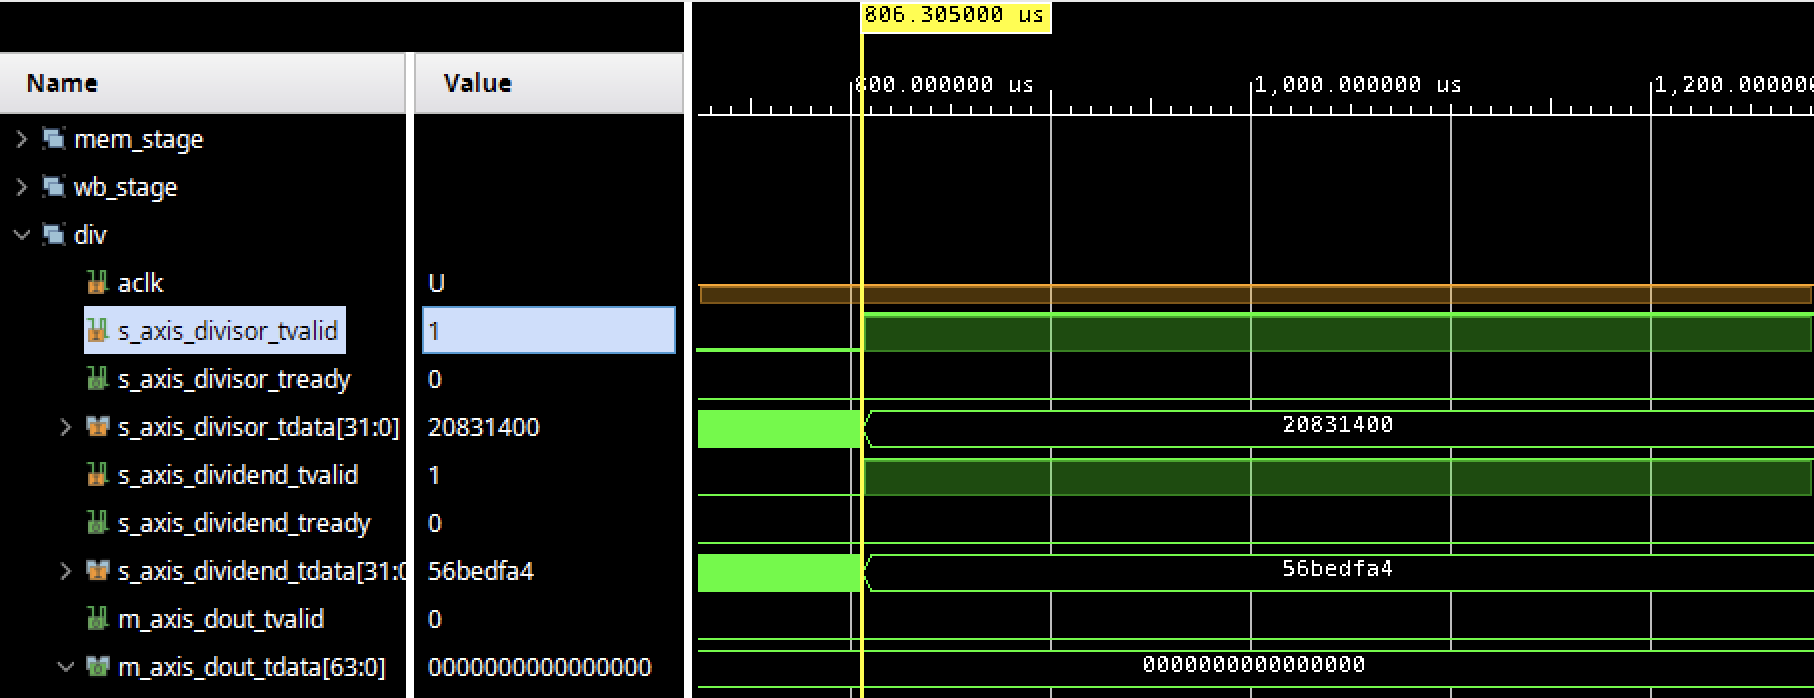
\includegraphics[width=0.7\linewidth]{no_aclk.png}
		\caption[no\_aclk]{除法器aclk信号悬空}
		\label{fig:noaclk}
	\end{figure}
	
	\paragraph{分析定位过程 \& 错误原因}\hfill
	
	因为错误为除法指令,去查看div模块如何出错,发现一个未赋值信号
	
	\paragraph{修正效果}\hfill
	
	只需要将div和divu模块接口全部定义就能避免这种问题
	
	\begin{lstlisting}[language=verilog]
	div_gen div(
		.aclk                   (clk),
		.s_axis_divisor_tdata   (alu_src2),
		.s_axis_dividend_tdata  (alu_src1),
		.s_axis_divisor_tready  (divisor_data_ready),
		.s_axis_dividend_tready (dividend_data_ready),
		.s_axis_divisor_tvalid  (div_data_valid),
		.s_axis_dividend_tvalid (div_data_valid),
		.m_axis_dout_tdata      (div_result),
		.m_axis_dout_tvalid     (div_res_valid)
	);
	\end{lstlisting}

	\paragraph{总结归纳}\hfill
	
	今后在遇到新的模块进行例化时要将需要操作的接口看全、注意类型和位宽,恰当使用。
	
	\subsubsection{错误\textbf{3:}除法器运算过程持续读取输入}
	
	\paragraph{错误现象}\hfill
	
	在遇到一个除法指令后,Valid和Ready信号仍然同时拉高,读取除法器输入并进行运算,接连输出多个结果。后一条乘法指令的结果被覆盖导致错误。
	
	\begin{figure}[h]
		\centering
		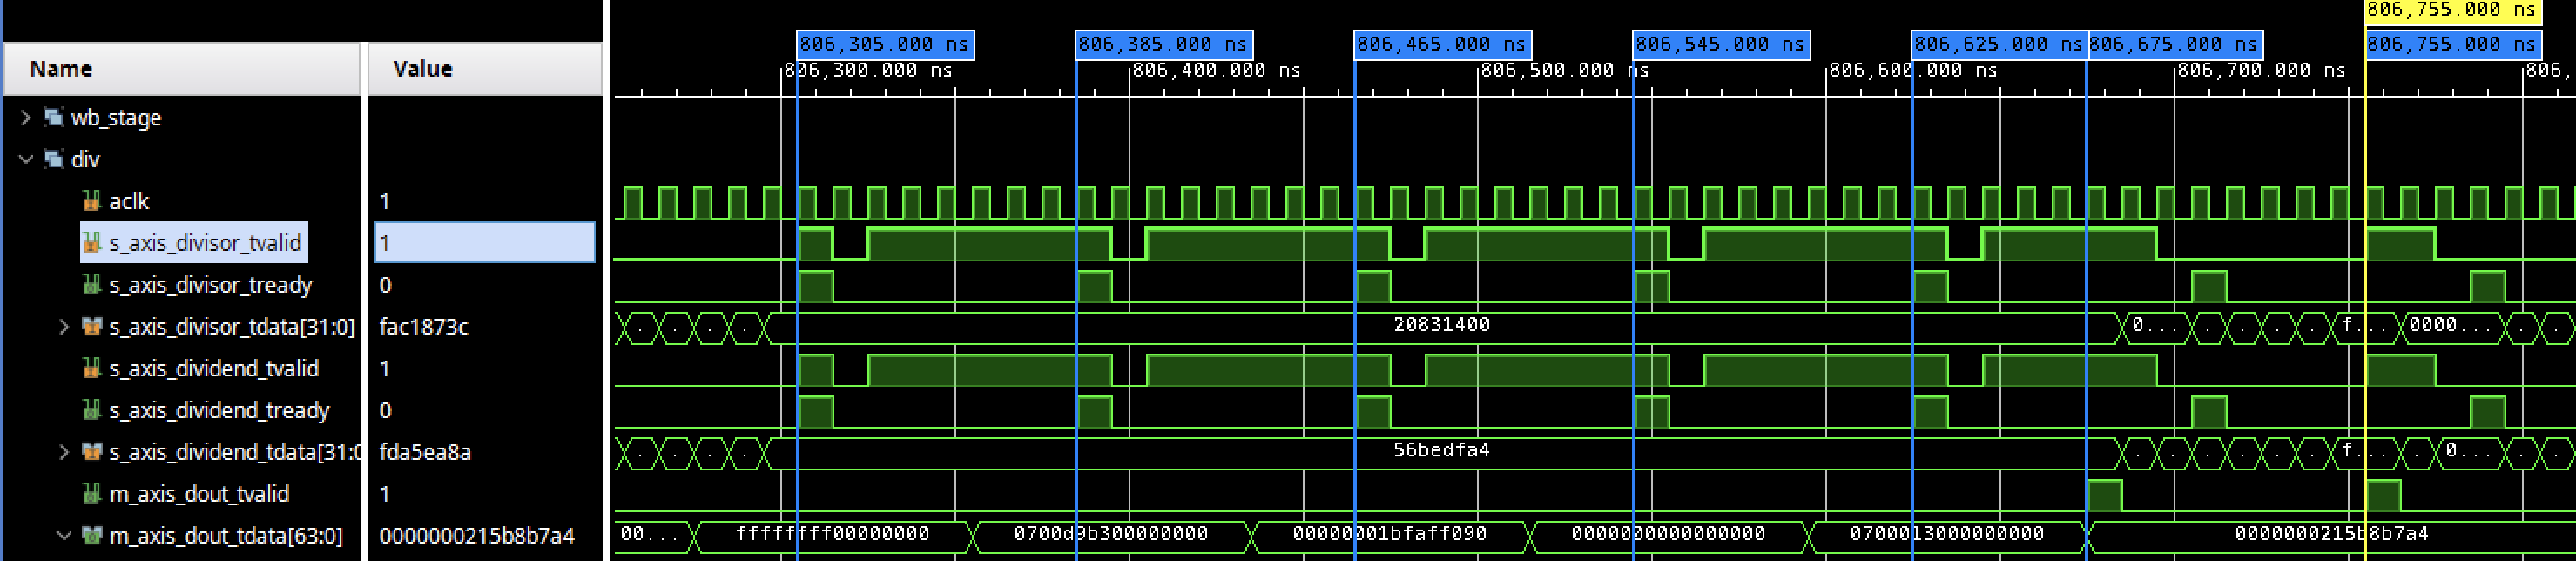
\includegraphics[width=1\linewidth]{valid_error.png}
		\caption[valid\_errpr]{除法器Valid信号设置错误}
		\label{fig:validerror}
	\end{figure}
	
	
	\paragraph{分析定位过程}\hfill
	
	最初留意的现象是连续两次除法运算时,后一条指令Valid和Ready信号已经读取成功,但并不开始运算。与此同时,除法器结果和前一条除法指令相同,并且m\_axis\_dout\_tvalid信号为高电平。
	
	多次尝试分析后才理解讲义的意思,Valid信号并不是每遇到一次Ready就拉低,而是在一次除法过程中只能拉高一次,否则会持续读取输入进行运算。
	
	\paragraph{错误原因}\hfill
	
	除法器Valid信号设置错误,在一次乘法指令中多次读取操作数输入进行运算,导致结果多次输出,可能会覆盖下一次乘法指令的结果。
	
	\begin{figure}[h]
		\centering
		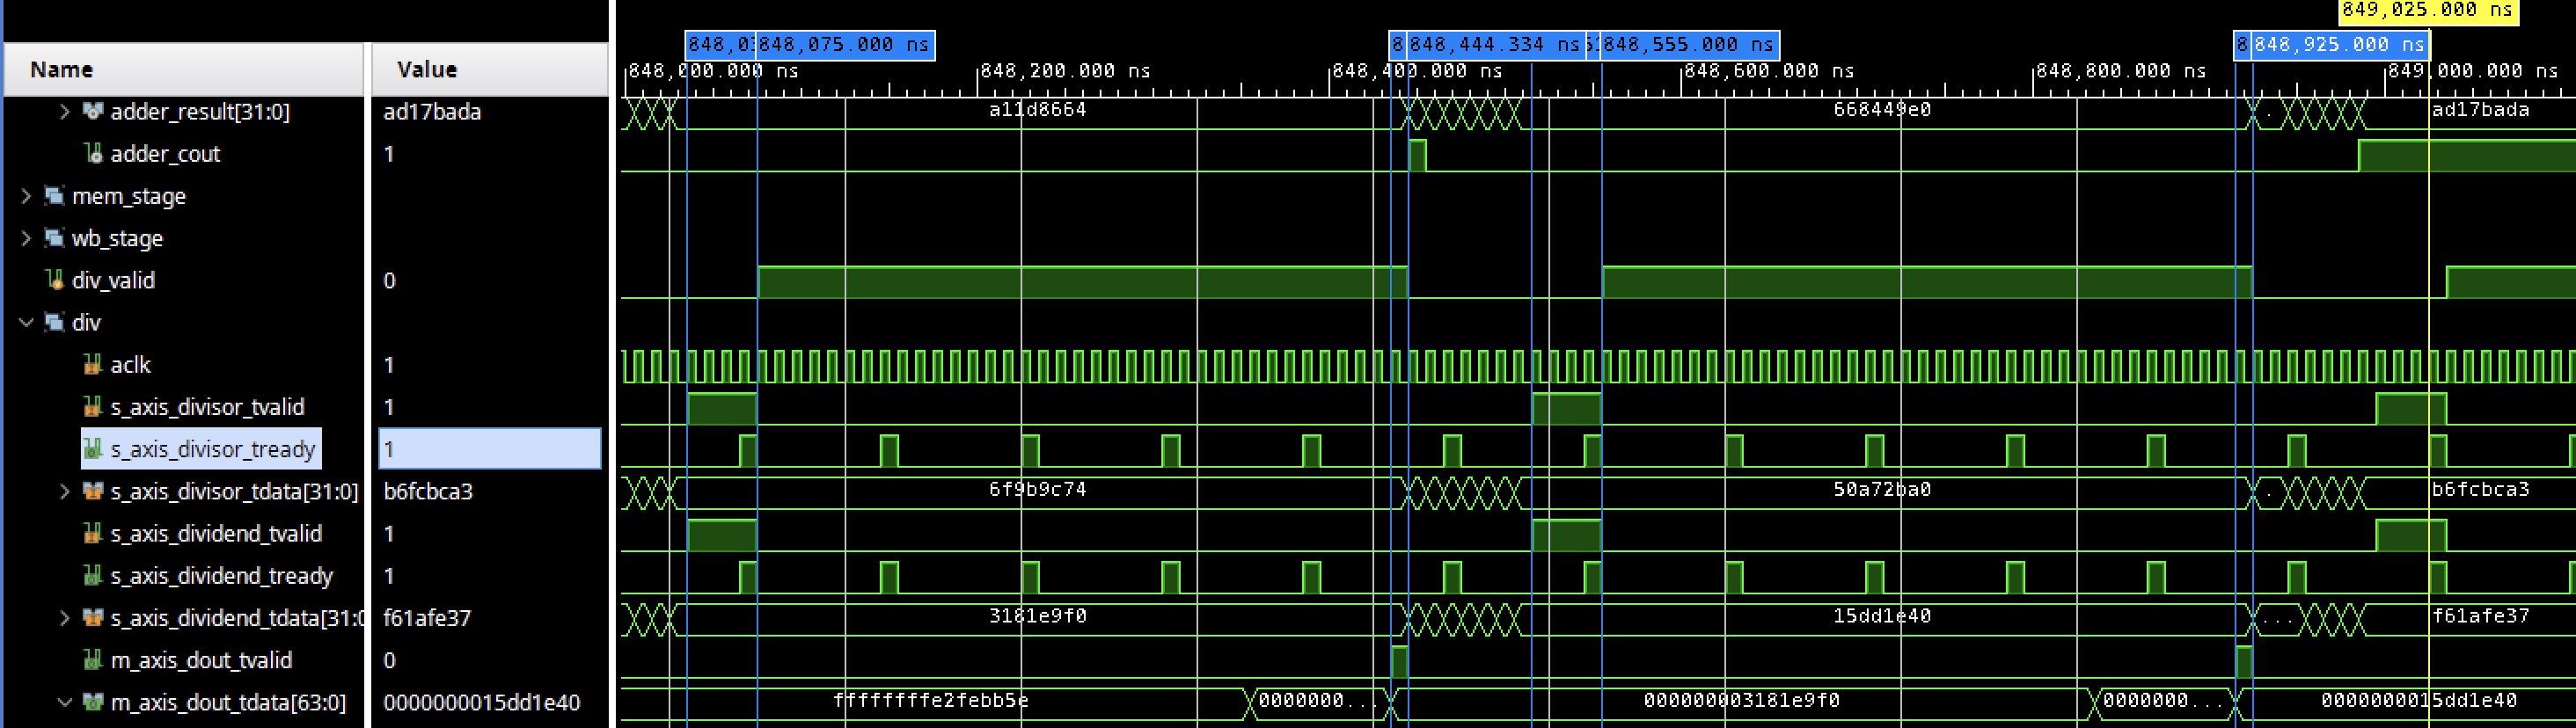
\includegraphics[width=1\linewidth]{valid_correct.png}
		\caption[Valid\_correct]{正确Valid输入信号效果}
		\label{fig:validcorrect}
	\end{figure}

	\paragraph{修正效果}\hfill
	
	采用新的变量div\_valid来表示除法开始到结束的过程,在此过程中除法器Valid输入只能在最开始拉高,紧接着持续拉低,修正代码如\ref{Valid_input} 中代码所示。修正后效果如下页所示。
	
	\paragraph{总结归纳}\hfill
	
	在遇到AXI总线多拍实现的部件时,需要对它输入输出接口的时序又深入了解,接合实现功能进行对接和赋值。
	
	\section{实验总结}
	
	运算式指令的主要实现复用此前实现的数据通路即可,特别注意乘除法导致的时序问题即可。
	
	时序满足上,乘法器使用Xilinx IP(即 * 号)时WNS为0.162\,ns,使用自行设计的单周期乘法器时WNS为0.073\,ns,将乘法器流水化后WNS(两拍完成乘法)为1.200\,ns。
	
\end{document}